% Archivo generado automaticamente por doc/tools/procesar_resultados.py
\section{Resultados autom\'aticos de pruebas}
\label{sec:resultados-automaticos}
\subsubsection{Escenario Prueba1 (20 dispositivos)}
\begin{figure}[!t]
  \centering
  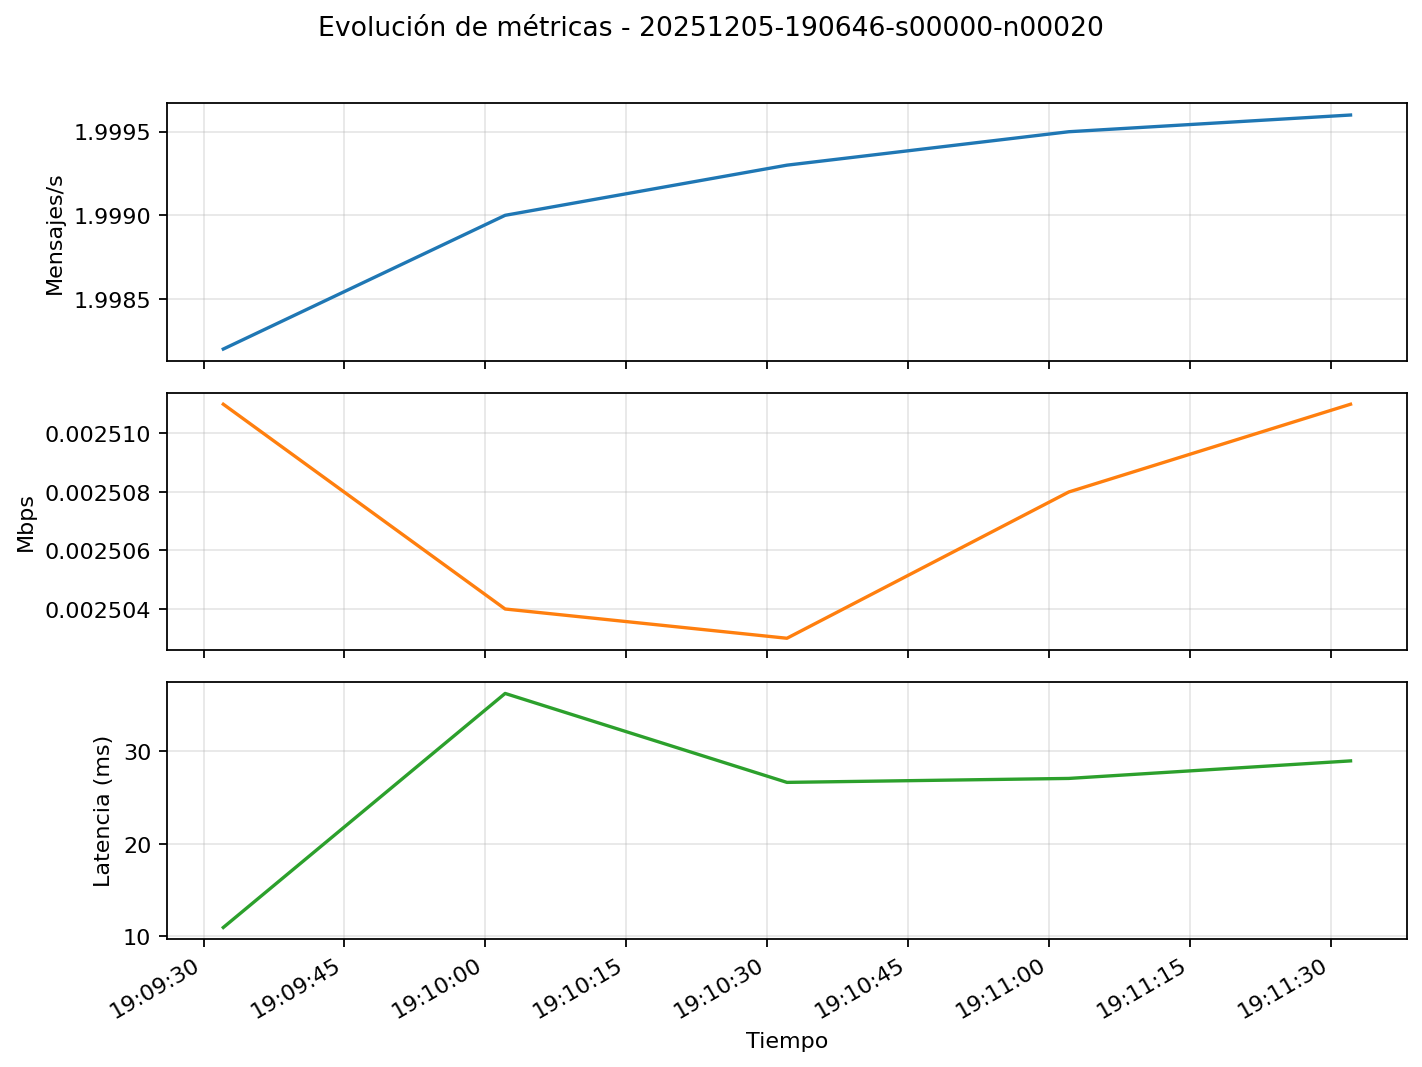
\includegraphics[width=\linewidth]{../data/metrics/reports/p1-20251205-190646-n20-overview.png}
  \caption{Evoluci\'on de m\'etricas del escenario Prueba1.}
  \label{fig:esc-prueba1}
\end{figure}
\begin{table}[!t]
  \centering
  \caption{Resumen del escenario Prueba1.}
  \label{tab:esc-prueba1}
  \begin{tabular}{@{}lrrrrr@{}}
    \toprule
    Sesi\'on & Nodos & Duraci\'on (s) & Mensajes & Lat. prom. (ms) & Throughput (msg/s)\\
    \midrule
    p1-20251205-190646-n20 & 20 & 150 & 300 & 25.989 & 1.999\\
    \bottomrule
  \end{tabular}
\end{table}
\paragraph{Conclusiones autom\'aticas}
\begin{itemize}
  \item Se ejercitaron aproximadamente 20 dispositivos.
  \item Entrega estable con p\'erdida <1\%.
  \item La latencia promedio se mantuvo baja para el escenario evaluado.
  \item El throughput medio fue de 2.00 msg/s.
\end{itemize}
\FloatBarrier
\subsubsection{Escenario Prueba2\_n100 (100 dispositivos)}
\begin{figure}[!t]
  \centering
  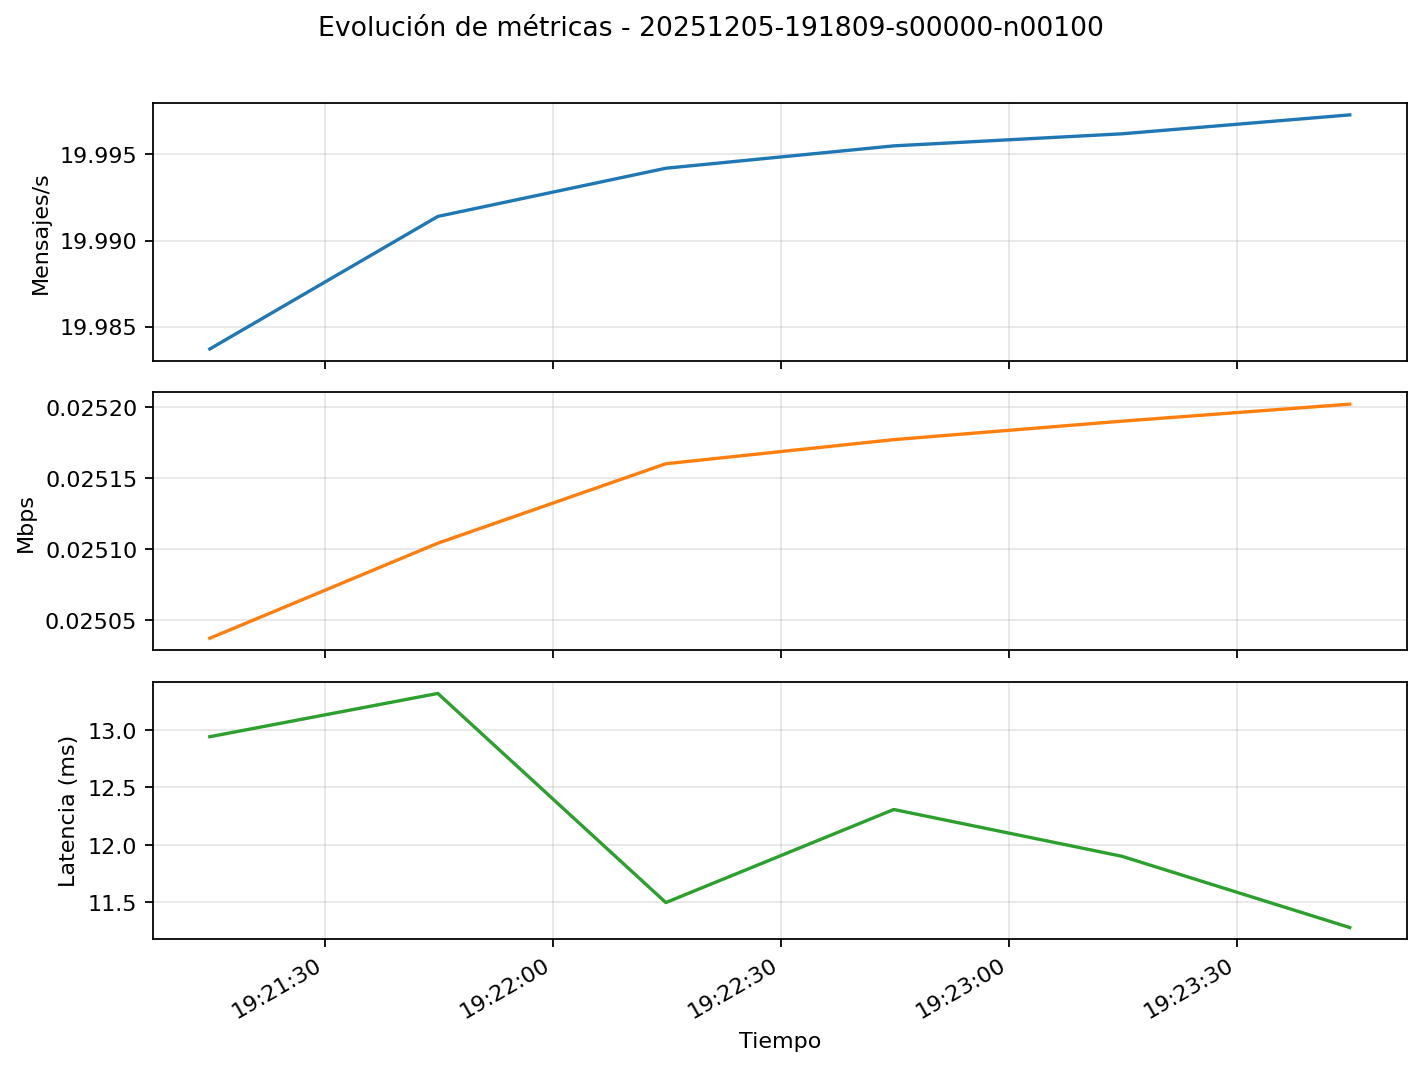
\includegraphics[width=\linewidth]{../data/metrics/reports/p2-n100-20251205-191809-n100-overview.png}
  \caption{Evoluci\'on de m\'etricas del escenario Prueba2\_n100.}
  \label{fig:esc-prueba2-n100}
\end{figure}
\begin{table}[!t]
  \centering
  \caption{Resumen del escenario Prueba2\_n100.}
  \label{tab:esc-prueba2-n100}
  \begin{tabular}{@{}lrrrrr@{}}
    \toprule
    Sesi\'on & Nodos & Duraci\'on (s) & Mensajes & Lat. prom. (ms) & Throughput (msg/s)\\
    \midrule
    p2-n100-20251205-191809-n100 & 100 & 180 & 3600 & 12.208 & 19.993\\
    \bottomrule
  \end{tabular}
\end{table}
\paragraph{Conclusiones autom\'aticas}
\begin{itemize}
  \item Se ejercitaron aproximadamente 100 dispositivos.
  \item Entrega estable con p\'erdida <1\%.
  \item La latencia promedio se mantuvo baja para el escenario evaluado.
  \item El throughput medio fue de 19.99 msg/s.
\end{itemize}
\FloatBarrier
\subsubsection{Escenario Prueba2\_n200 (200 dispositivos)}
\begin{figure}[!t]
  \centering
  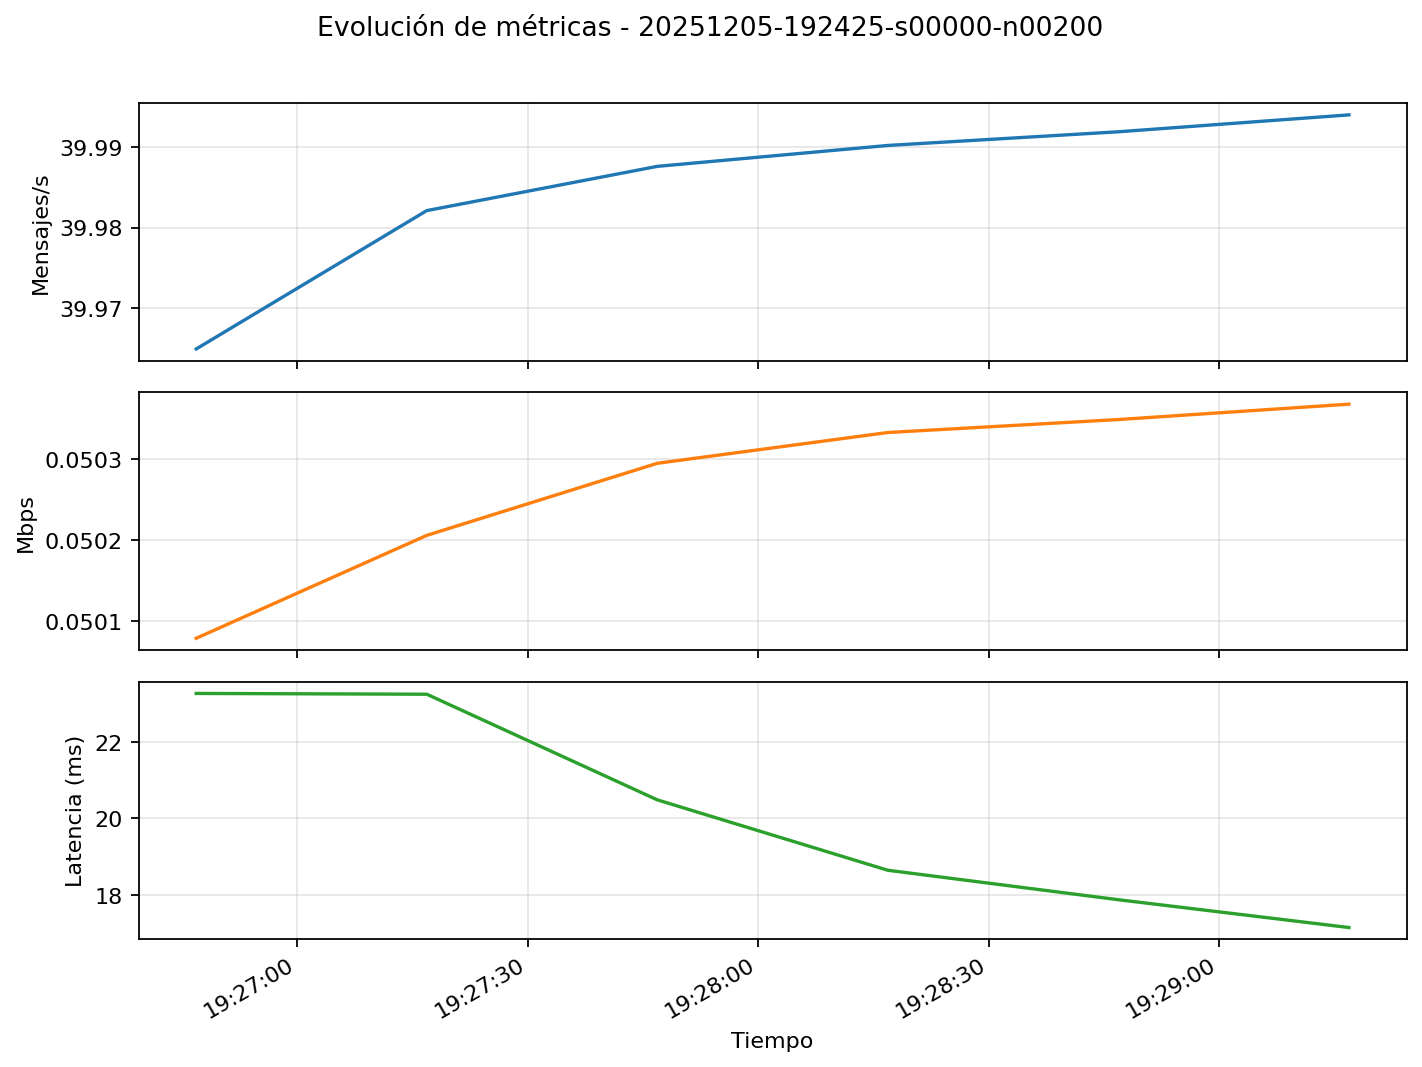
\includegraphics[width=\linewidth]{../data/metrics/reports/p2-n200-20251205-192425-n200-overview.png}
  \caption{Evoluci\'on de m\'etricas del escenario Prueba2\_n200.}
  \label{fig:esc-prueba2-n200}
\end{figure}
\begin{table}[!t]
  \centering
  \caption{Resumen del escenario Prueba2\_n200.}
  \label{tab:esc-prueba2-n200}
  \begin{tabular}{@{}lrrrrr@{}}
    \toprule
    Sesi\'on & Nodos & Duraci\'on (s) & Mensajes & Lat. prom. (ms) & Throughput (msg/s)\\
    \midrule
    p2-n200-20251205-192425-n200 & 200 & 180 & 7200 & 20.109 & 39.985\\
    \bottomrule
  \end{tabular}
\end{table}
\paragraph{Conclusiones autom\'aticas}
\begin{itemize}
  \item Se ejercitaron aproximadamente 200 dispositivos.
  \item Entrega estable con p\'erdida <1\%.
  \item La latencia promedio se mantuvo baja para el escenario evaluado.
  \item El throughput medio fue de 39.99 msg/s.
\end{itemize}
\FloatBarrier
\subsubsection{Escenario Prueba2\_n400 (400 dispositivos)}
\begin{figure}[!t]
  \centering
  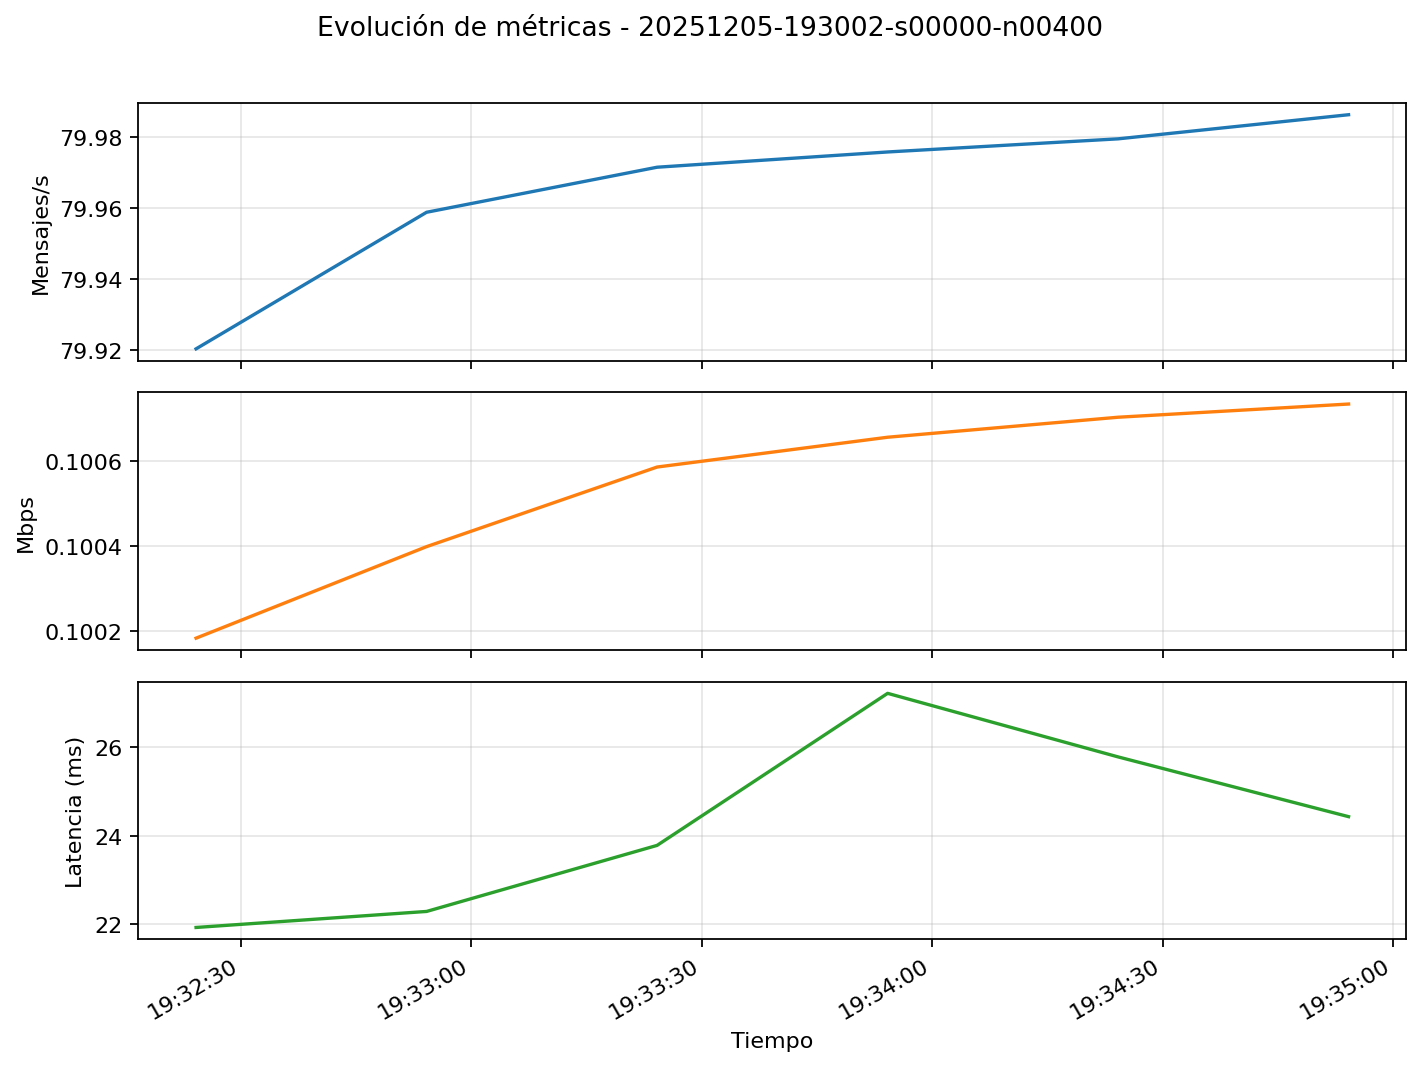
\includegraphics[width=\linewidth]{../data/metrics/reports/p2-n400-20251205-193002-n400-overview.png}
  \caption{Evoluci\'on de m\'etricas del escenario Prueba2\_n400.}
  \label{fig:esc-prueba2-n400}
\end{figure}
\begin{table}[!t]
  \centering
  \caption{Resumen del escenario Prueba2\_n400.}
  \label{tab:esc-prueba2-n400}
  \begin{tabular}{@{}lrrrrr@{}}
    \toprule
    Sesi\'on & Nodos & Duraci\'on (s) & Mensajes & Lat. prom. (ms) & Throughput (msg/s)\\
    \midrule
    p2-n400-20251205-193002-n400 & 400 & 180 & 14400 & 24.234 & 79.965\\
    \bottomrule
  \end{tabular}
\end{table}
\paragraph{Conclusiones autom\'aticas}
\begin{itemize}
  \item Se ejercitaron aproximadamente 400 dispositivos.
  \item Entrega estable con p\'erdida <1\%.
  \item La latencia promedio se mantuvo baja para el escenario evaluado.
  \item El throughput medio fue de 79.97 msg/s.
\end{itemize}
\FloatBarrier
\subsubsection{Escenario Prueba2\_n50 (50 dispositivos)}
\begin{figure}[!t]
  \centering
  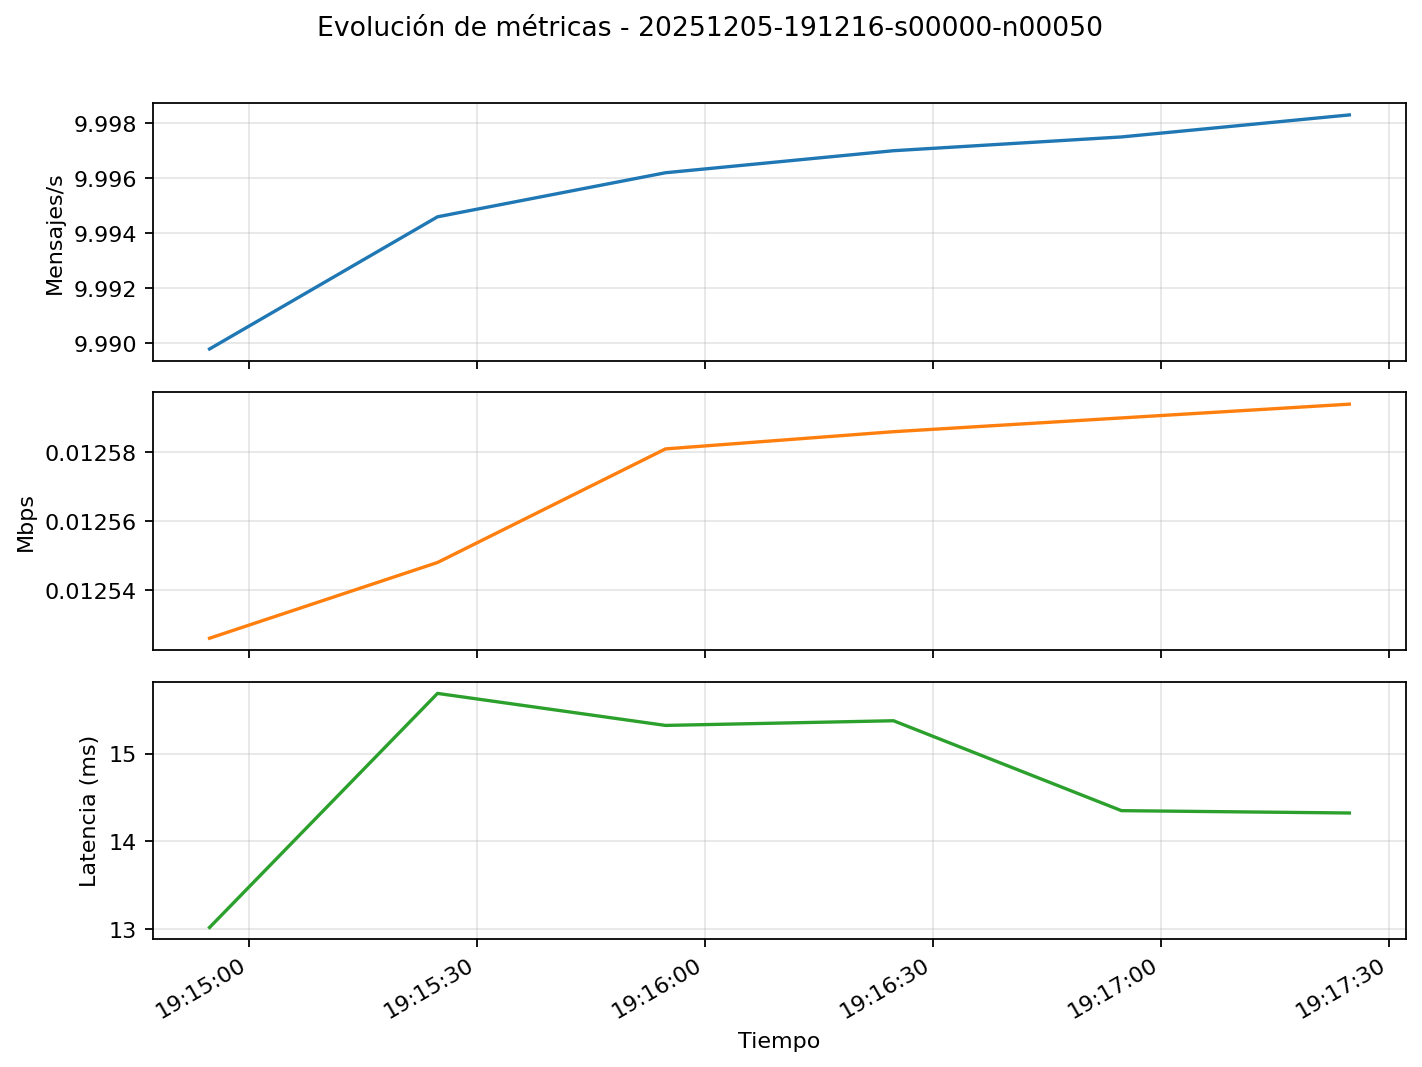
\includegraphics[width=\linewidth]{../data/metrics/reports/p2-n50-20251205-191216-n50-overview.png}
  \caption{Evoluci\'on de m\'etricas del escenario Prueba2\_n50.}
  \label{fig:esc-prueba2-n50}
\end{figure}
\begin{table}[!t]
  \centering
  \caption{Resumen del escenario Prueba2\_n50.}
  \label{tab:esc-prueba2-n50}
  \begin{tabular}{@{}lrrrrr@{}}
    \toprule
    Sesi\'on & Nodos & Duraci\'on (s) & Mensajes & Lat. prom. (ms) & Throughput (msg/s)\\
    \midrule
    p2-n50-20251205-191216-n50 & 50 & 180 & 1800 & 14.679 & 9.996\\
    \bottomrule
  \end{tabular}
\end{table}
\paragraph{Conclusiones autom\'aticas}
\begin{itemize}
  \item Se ejercitaron aproximadamente 50 dispositivos.
  \item Entrega estable con p\'erdida <1\%.
  \item La latencia promedio se mantuvo baja para el escenario evaluado.
  \item El throughput medio fue de 10.00 msg/s.
\end{itemize}
\FloatBarrier
\subsubsection{Escenario Prueba3\_int1 (200 dispositivos)}
\begin{figure}[!t]
  \centering
  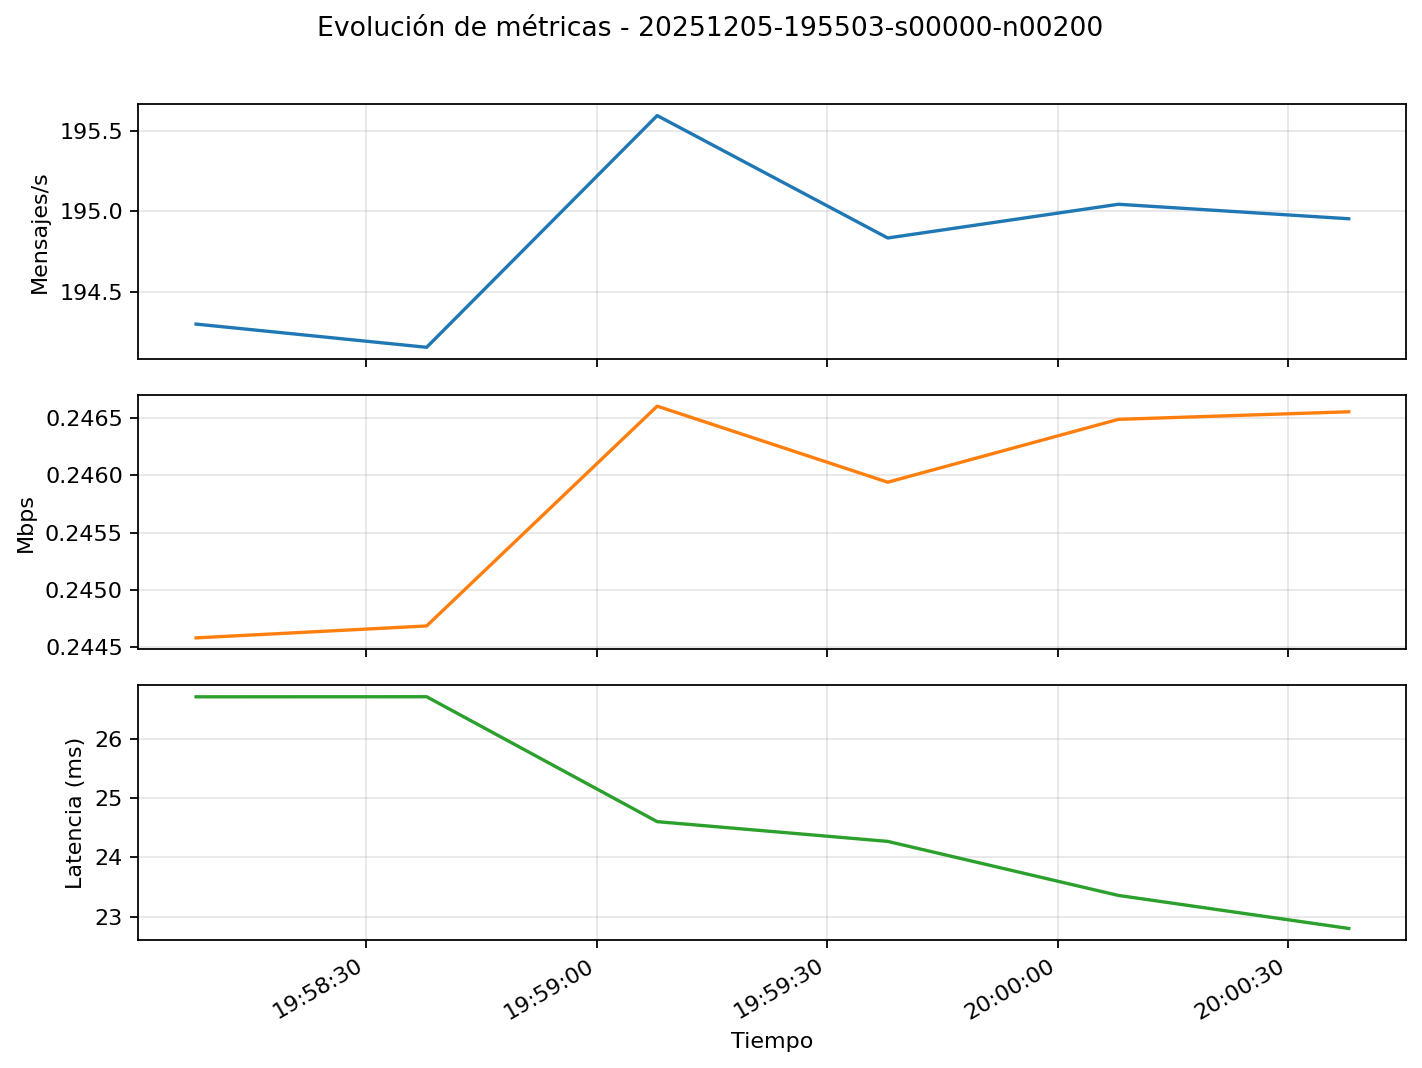
\includegraphics[width=\linewidth]{../data/metrics/reports/p3-int1-20251205-195503-n200-overview.png}
  \caption{Evoluci\'on de m\'etricas del escenario Prueba3\_int1.}
  \label{fig:esc-prueba3-int1}
\end{figure}
\begin{table}[!t]
  \centering
  \caption{Resumen del escenario Prueba3\_int1.}
  \label{tab:esc-prueba3-int1}
  \begin{tabular}{@{}lrrrrr@{}}
    \toprule
    Sesi\'on & Nodos & Duraci\'on (s) & Mensajes & Lat. prom. (ms) & Throughput (msg/s)\\
    \midrule
    p3-int1-20251205-195503-n200 & 200 & 180 & 35097 & 24.742 & 194.813\\
    \bottomrule
  \end{tabular}
\end{table}
\paragraph{Conclusiones autom\'aticas}
\begin{itemize}
  \item Se ejercitaron aproximadamente 200 dispositivos.
  \item Entrega estable con p\'erdida <1\%.
  \item La latencia promedio se mantuvo baja para el escenario evaluado.
  \item El throughput medio fue de 194.81 msg/s.
\end{itemize}
\FloatBarrier
\subsubsection{Escenario Prueba3\_int10 (200 dispositivos)}
\begin{figure}[!t]
  \centering
  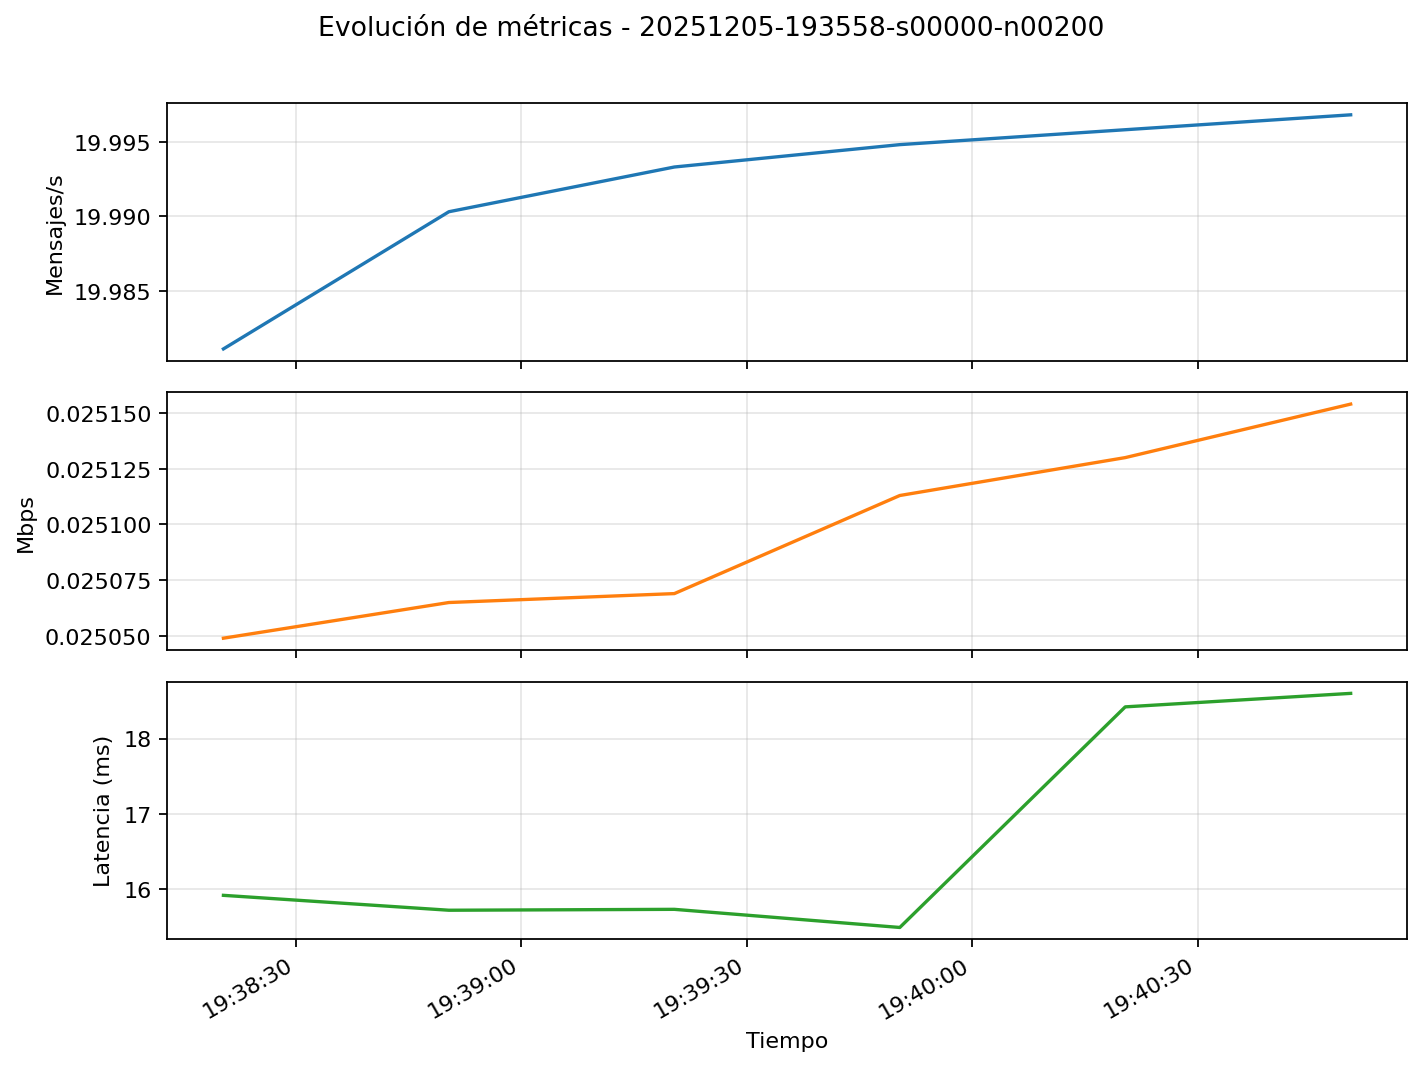
\includegraphics[width=\linewidth]{../data/metrics/reports/p3-int10-20251205-193558-n200-overview.png}
  \caption{Evoluci\'on de m\'etricas del escenario Prueba3\_int10.}
  \label{fig:esc-prueba3-int10}
\end{figure}
\begin{table}[!t]
  \centering
  \caption{Resumen del escenario Prueba3\_int10.}
  \label{tab:esc-prueba3-int10}
  \begin{tabular}{@{}lrrrrr@{}}
    \toprule
    Sesi\'on & Nodos & Duraci\'on (s) & Mensajes & Lat. prom. (ms) & Throughput (msg/s)\\
    \midrule
    p3-int10-20251205-193558-n200 & 200 & 180 & 3600 & 16.648 & 19.992\\
    \bottomrule
  \end{tabular}
\end{table}
\paragraph{Conclusiones autom\'aticas}
\begin{itemize}
  \item Se ejercitaron aproximadamente 200 dispositivos.
  \item Entrega estable con p\'erdida <1\%.
  \item La latencia promedio se mantuvo baja para el escenario evaluado.
  \item El throughput medio fue de 19.99 msg/s.
\end{itemize}
\FloatBarrier
\subsubsection{Escenario Prueba3\_int2 (200 dispositivos)}
\begin{figure}[!t]
  \centering
  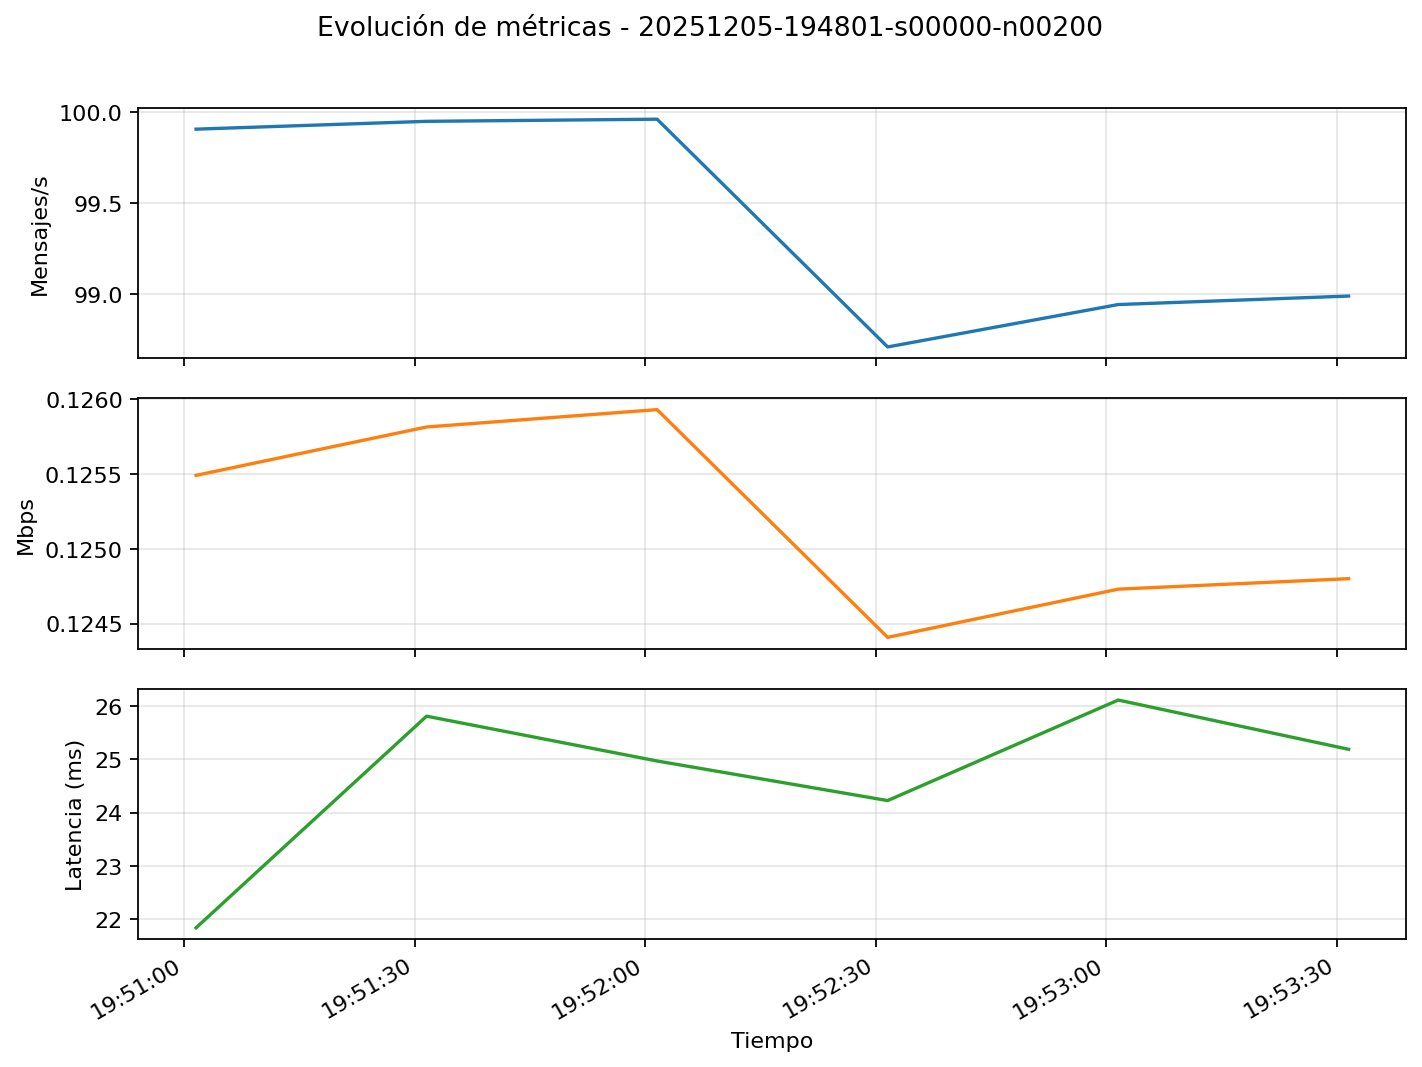
\includegraphics[width=\linewidth]{../data/metrics/reports/p3-int2-20251205-194801-n200-overview.png}
  \caption{Evoluci\'on de m\'etricas del escenario Prueba3\_int2.}
  \label{fig:esc-prueba3-int2}
\end{figure}
\begin{table}[!t]
  \centering
  \caption{Resumen del escenario Prueba3\_int2.}
  \label{tab:esc-prueba3-int2}
  \begin{tabular}{@{}lrrrrr@{}}
    \toprule
    Sesi\'on & Nodos & Duraci\'on (s) & Mensajes & Lat. prom. (ms) & Throughput (msg/s)\\
    \midrule
    p3-int2-20251205-194801-n200 & 200 & 180 & 17821 & 24.690 & 99.410\\
    \bottomrule
  \end{tabular}
\end{table}
\paragraph{Conclusiones autom\'aticas}
\begin{itemize}
  \item Se ejercitaron aproximadamente 200 dispositivos.
  \item Entrega estable con p\'erdida <1\%.
  \item La latencia promedio se mantuvo baja para el escenario evaluado.
  \item El throughput medio fue de 99.41 msg/s.
\end{itemize}
\FloatBarrier
\subsubsection{Escenario Prueba3\_int5 (200 dispositivos)}
\begin{figure}[!t]
  \centering
  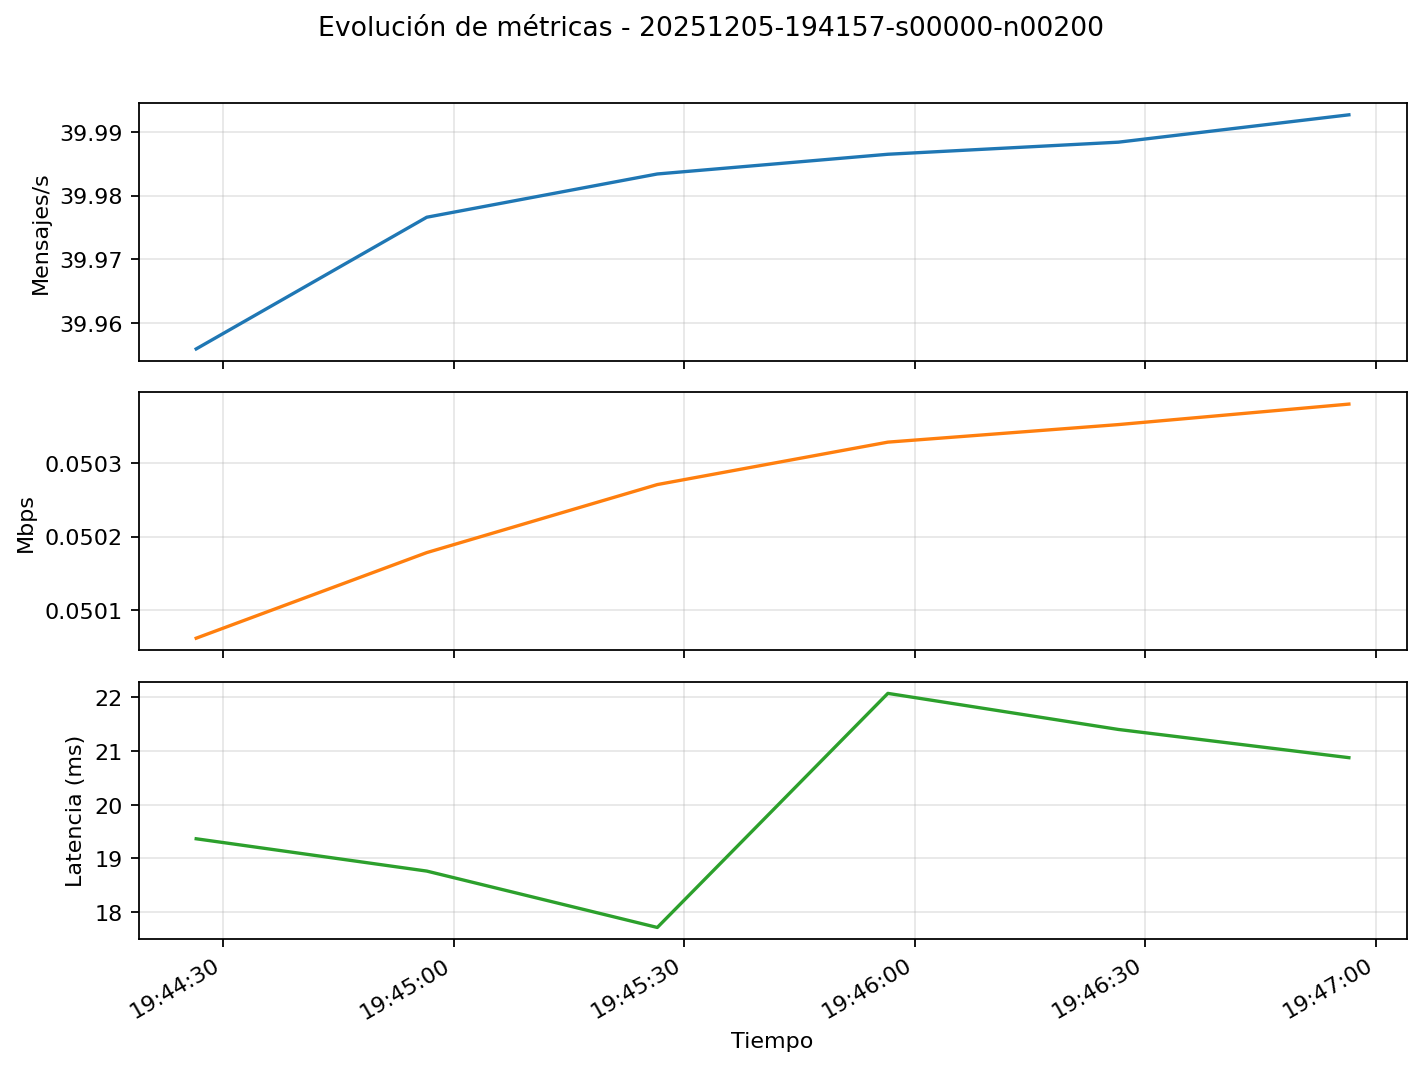
\includegraphics[width=\linewidth]{../data/metrics/reports/p3-int5-20251205-194157-n200-overview.png}
  \caption{Evoluci\'on de m\'etricas del escenario Prueba3\_int5.}
  \label{fig:esc-prueba3-int5}
\end{figure}
\begin{table}[!t]
  \centering
  \caption{Resumen del escenario Prueba3\_int5.}
  \label{tab:esc-prueba3-int5}
  \begin{tabular}{@{}lrrrrr@{}}
    \toprule
    Sesi\'on & Nodos & Duraci\'on (s) & Mensajes & Lat. prom. (ms) & Throughput (msg/s)\\
    \midrule
    p3-int5-20251205-194157-n200 & 200 & 180 & 7200 & 20.031 & 39.981\\
    \bottomrule
  \end{tabular}
\end{table}
\paragraph{Conclusiones autom\'aticas}
\begin{itemize}
  \item Se ejercitaron aproximadamente 200 dispositivos.
  \item Entrega estable con p\'erdida <1\%.
  \item La latencia promedio se mantuvo baja para el escenario evaluado.
  \item El throughput medio fue de 39.98 msg/s.
\end{itemize}
\FloatBarrier
\subsubsection{Escenario Prueba4\_large (200 dispositivos)}
\begin{figure}[!t]
  \centering
  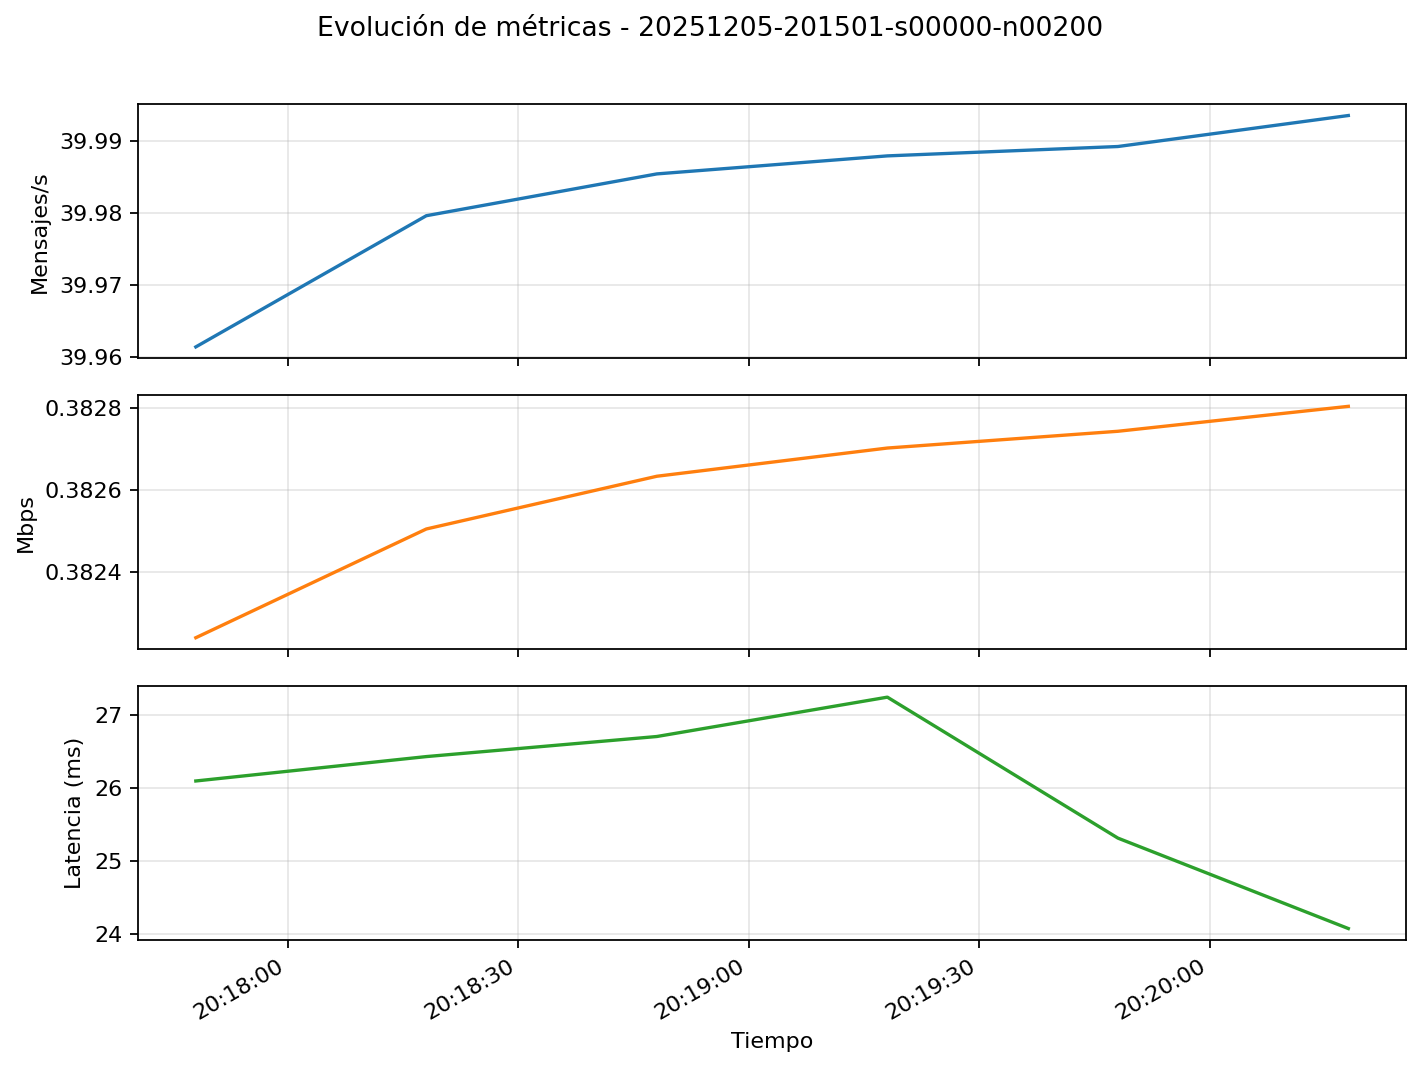
\includegraphics[width=\linewidth]{../data/metrics/reports/p4-l-20251205-201501-n200-overview.png}
  \caption{Evoluci\'on de m\'etricas del escenario Prueba4\_large.}
  \label{fig:esc-prueba4-large}
\end{figure}
\begin{table}[!t]
  \centering
  \caption{Resumen del escenario Prueba4\_large.}
  \label{tab:esc-prueba4-large}
  \begin{tabular}{@{}lrrrrr@{}}
    \toprule
    Sesi\'on & Nodos & Duraci\'on (s) & Mensajes & Lat. prom. (ms) & Throughput (msg/s)\\
    \midrule
    p4-l-20251205-201501-n200 & 200 & 180 & 7200 & 25.977 & 39.983\\
    \bottomrule
  \end{tabular}
\end{table}
\paragraph{Conclusiones autom\'aticas}
\begin{itemize}
  \item Se ejercitaron aproximadamente 200 dispositivos.
  \item Entrega estable con p\'erdida <1\%.
  \item La latencia promedio se mantuvo baja para el escenario evaluado.
  \item El throughput medio fue de 39.98 msg/s.
\end{itemize}
\FloatBarrier
\subsubsection{Escenario Prueba4\_medium (200 dispositivos)}
\begin{figure}[!t]
  \centering
  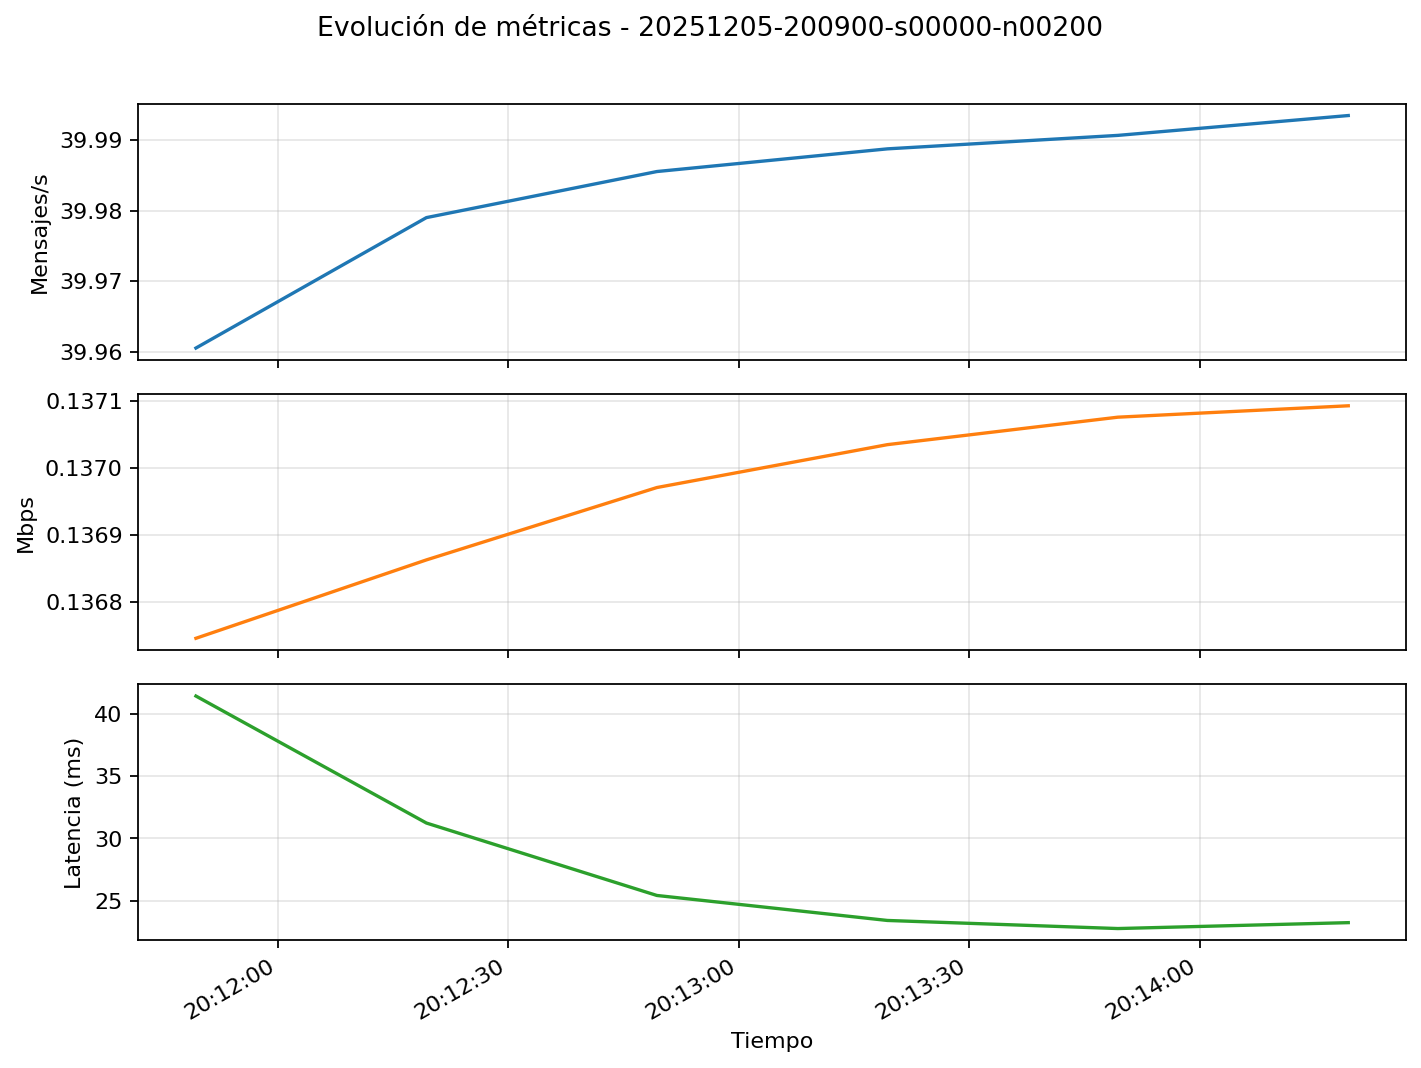
\includegraphics[width=\linewidth]{../data/metrics/reports/p4-m-20251205-200900-n200-overview.png}
  \caption{Evoluci\'on de m\'etricas del escenario Prueba4\_medium.}
  \label{fig:esc-prueba4-medium}
\end{figure}
\begin{table}[!t]
  \centering
  \caption{Resumen del escenario Prueba4\_medium.}
  \label{tab:esc-prueba4-medium}
  \begin{tabular}{@{}lrrrrr@{}}
    \toprule
    Sesi\'on & Nodos & Duraci\'on (s) & Mensajes & Lat. prom. (ms) & Throughput (msg/s)\\
    \midrule
    p4-m-20251205-200900-n200 & 200 & 180 & 7200 & 27.916 & 39.983\\
    \bottomrule
  \end{tabular}
\end{table}
\paragraph{Conclusiones autom\'aticas}
\begin{itemize}
  \item Se ejercitaron aproximadamente 200 dispositivos.
  \item Entrega estable con p\'erdida <1\%.
  \item La latencia promedio se mantuvo baja para el escenario evaluado.
  \item El throughput medio fue de 39.98 msg/s.
\end{itemize}
\FloatBarrier
\subsubsection{Escenario Prueba4\_small (200 dispositivos)}
\begin{figure}[!t]
  \centering
  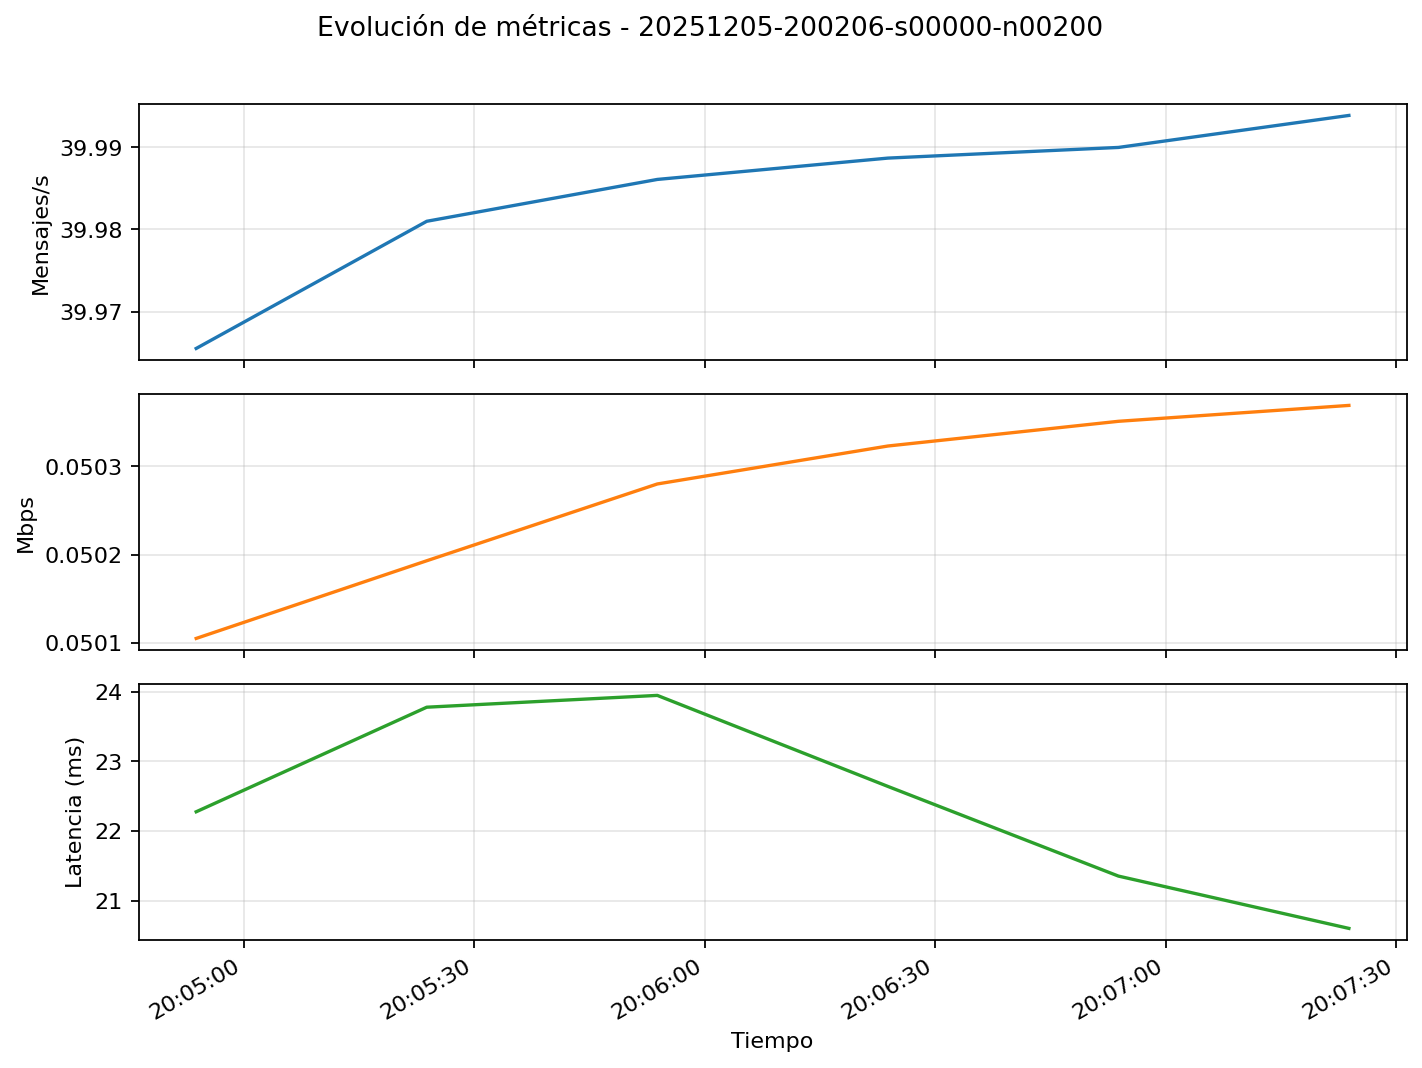
\includegraphics[width=\linewidth]{../data/metrics/reports/p4-s-20251205-200206-n200-overview.png}
  \caption{Evoluci\'on de m\'etricas del escenario Prueba4\_small.}
  \label{fig:esc-prueba4-small}
\end{figure}
\begin{table}[!t]
  \centering
  \caption{Resumen del escenario Prueba4\_small.}
  \label{tab:esc-prueba4-small}
  \begin{tabular}{@{}lrrrrr@{}}
    \toprule
    Sesi\'on & Nodos & Duraci\'on (s) & Mensajes & Lat. prom. (ms) & Throughput (msg/s)\\
    \midrule
    p4-s-20251205-200206-n200 & 200 & 180 & 7200 & 22.435 & 39.984\\
    \bottomrule
  \end{tabular}
\end{table}
\paragraph{Conclusiones autom\'aticas}
\begin{itemize}
  \item Se ejercitaron aproximadamente 200 dispositivos.
  \item Entrega estable con p\'erdida <1\%.
  \item La latencia promedio se mantuvo baja para el escenario evaluado.
  \item El throughput medio fue de 39.98 msg/s.
\end{itemize}
\FloatBarrier
\subsubsection{Escenario Prueba5\_con\_rate\_limit (200 dispositivos)}
\begin{figure}[!t]
  \centering
  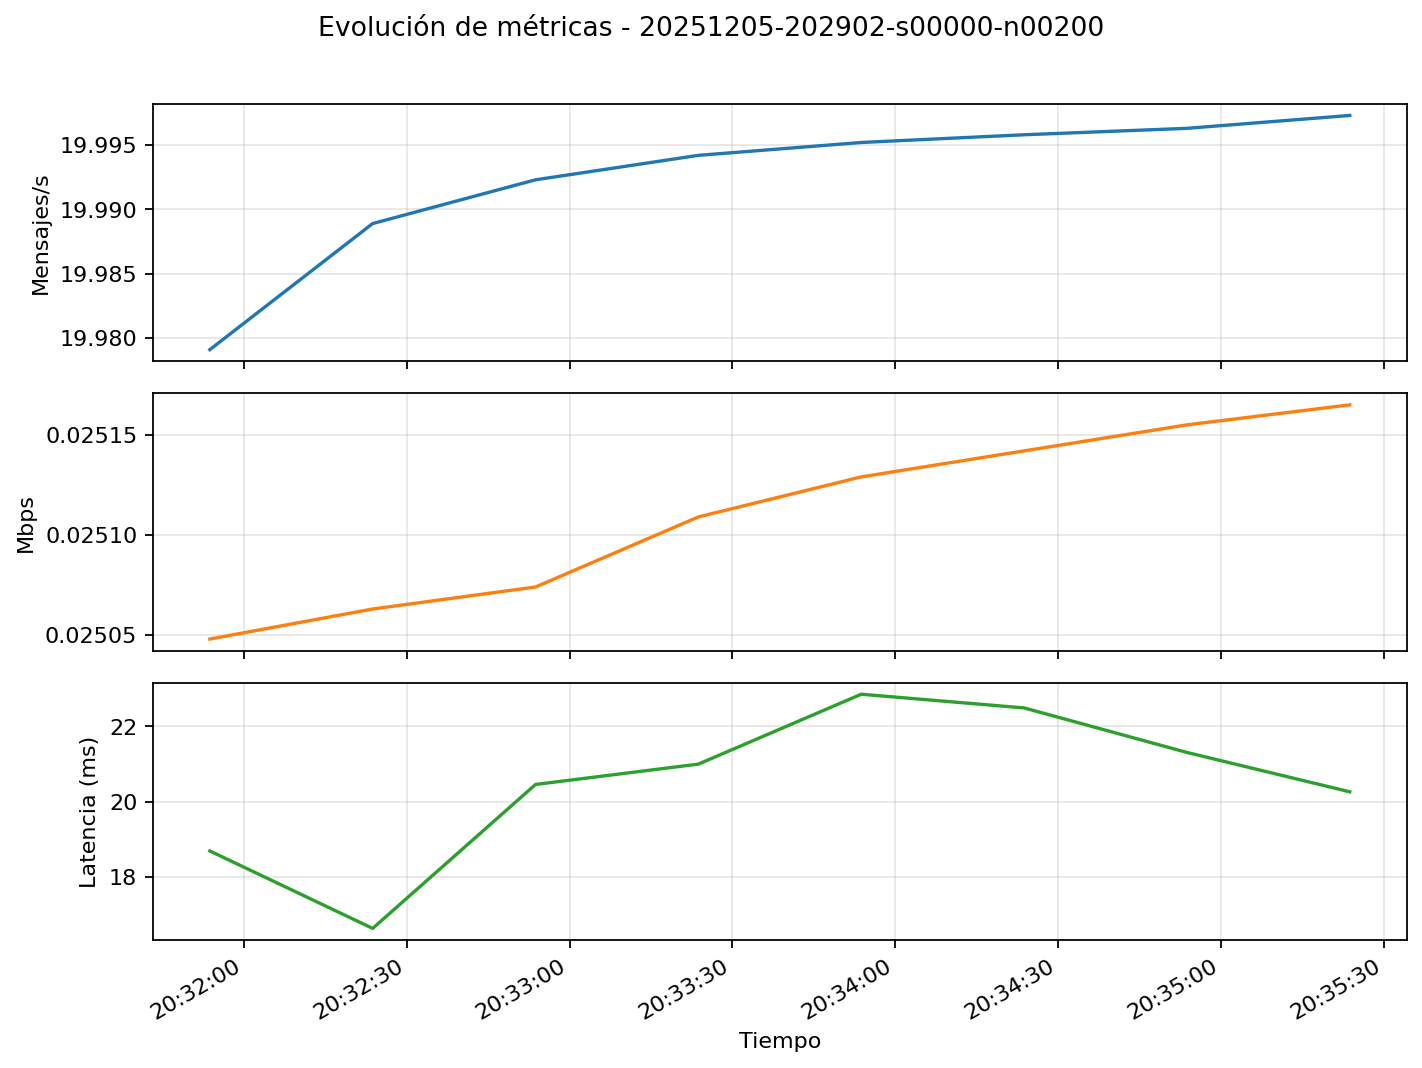
\includegraphics[width=\linewidth]{../data/metrics/reports/p5-rl-20251205-202902-n200-overview.png}
  \caption{Evoluci\'on de m\'etricas del escenario Prueba5\_con\_rate\_limit.}
  \label{fig:esc-prueba5-con-rate-limit}
\end{figure}
\begin{table}[!t]
  \centering
  \caption{Resumen del escenario Prueba5\_con\_rate\_limit.}
  \label{tab:esc-prueba5-con-rate-limit}
  \begin{tabular}{@{}lrrrrr@{}}
    \toprule
    Sesi\'on & Nodos & Duraci\'on (s) & Mensajes & Lat. prom. (ms) & Throughput (msg/s)\\
    \midrule
    p5-rl-20251205-202902-n200 & 200 & 240 & 4800 & 20.460 & 19.992\\
    \bottomrule
  \end{tabular}
\end{table}
\paragraph{Conclusiones autom\'aticas}
\begin{itemize}
  \item Se ejercitaron aproximadamente 200 dispositivos.
  \item Entrega estable con p\'erdida <1\%.
  \item La latencia promedio se mantuvo baja para el escenario evaluado.
  \item El throughput medio fue de 19.99 msg/s.
\end{itemize}
\FloatBarrier
\subsubsection{Escenario Prueba5\_sin\_aggregate (200 dispositivos)}
\begin{figure}[!t]
  \centering
  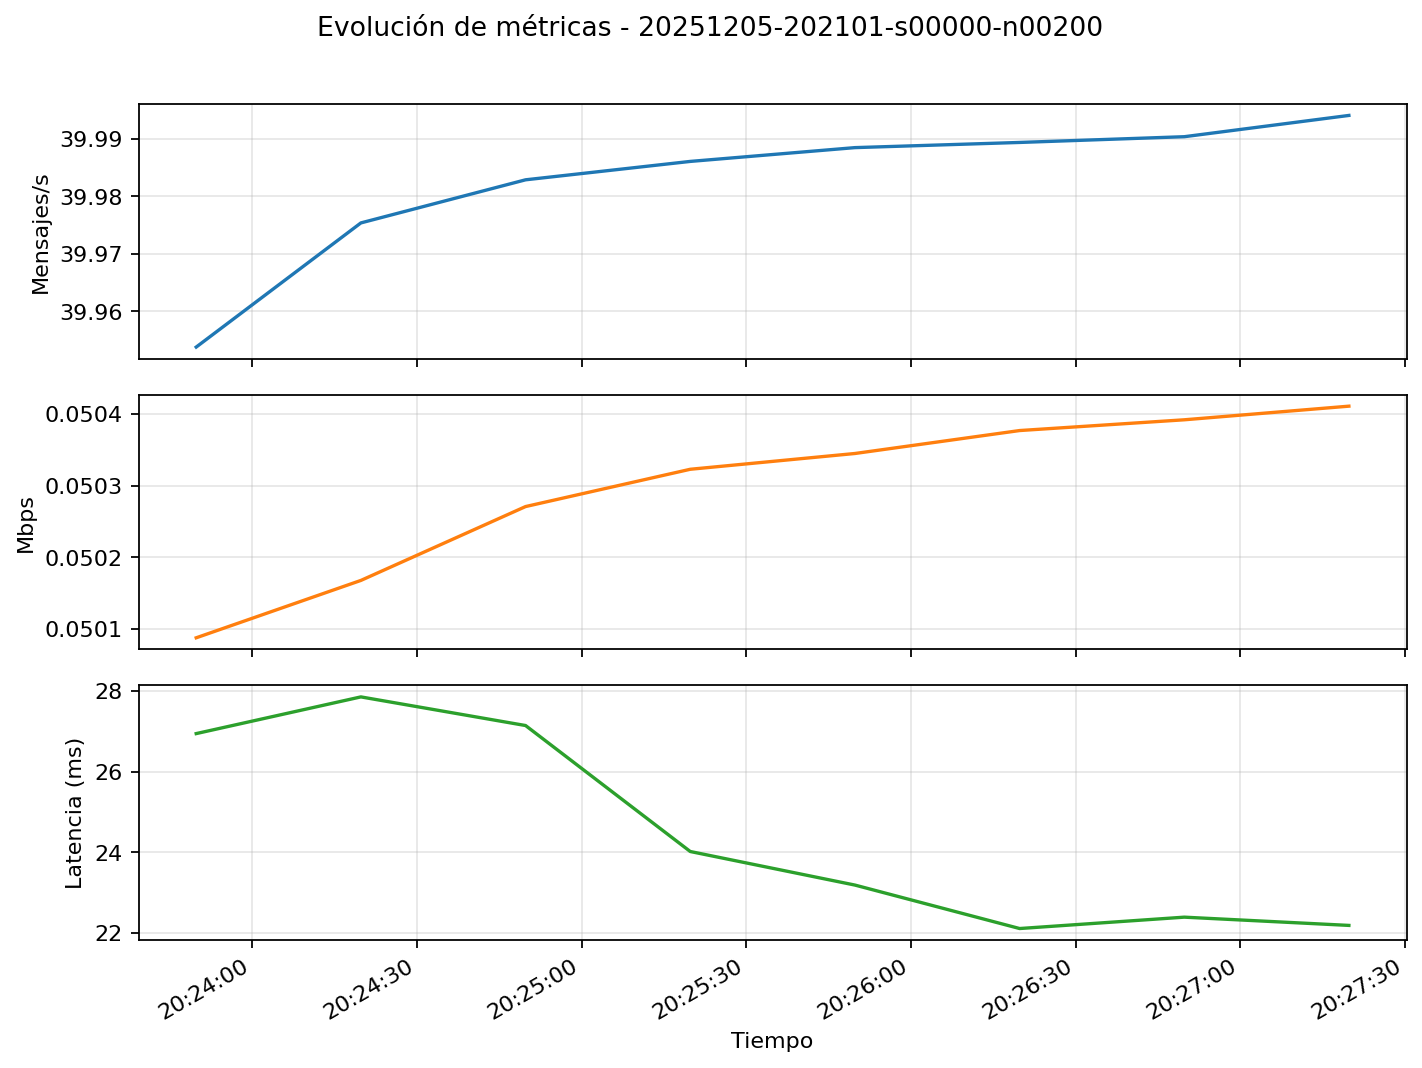
\includegraphics[width=\linewidth]{../data/metrics/reports/p5-sa-20251205-202101-n200-overview.png}
  \caption{Evoluci\'on de m\'etricas del escenario Prueba5\_sin\_aggregate.}
  \label{fig:esc-prueba5-sin-aggregate}
\end{figure}
\begin{table}[!t]
  \centering
  \caption{Resumen del escenario Prueba5\_sin\_aggregate.}
  \label{tab:esc-prueba5-sin-aggregate}
  \begin{tabular}{@{}lrrrrr@{}}
    \toprule
    Sesi\'on & Nodos & Duraci\'on (s) & Mensajes & Lat. prom. (ms) & Throughput (msg/s)\\
    \midrule
    p5-sa-20251205-202101-n200 & 200 & 240 & 9600 & 24.481 & 39.983\\
    \bottomrule
  \end{tabular}
\end{table}
\paragraph{Conclusiones autom\'aticas}
\begin{itemize}
  \item Se ejercitaron aproximadamente 200 dispositivos.
  \item Entrega estable con p\'erdida <1\%.
  \item La latencia promedio se mantuvo baja para el escenario evaluado.
  \item El throughput medio fue de 39.98 msg/s.
\end{itemize}
\FloatBarrier
\subsubsection{Escenario Prueba6 (400 dispositivos)}
\begin{figure}[!t]
  \centering
  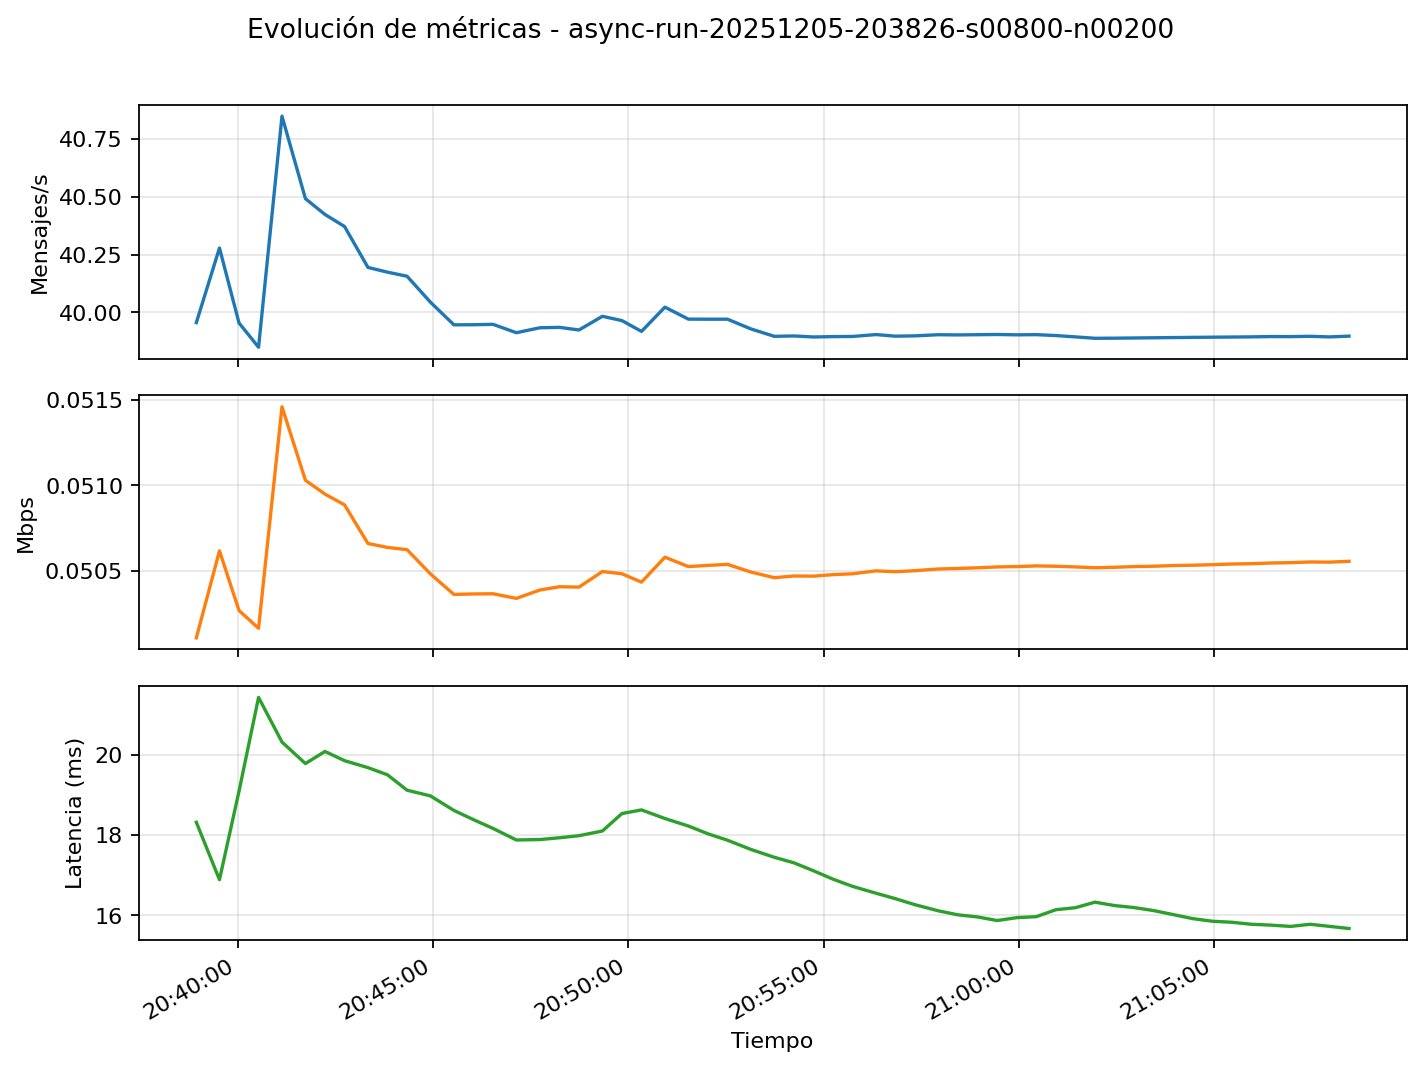
\includegraphics[width=\linewidth]{../data/metrics/reports/p6-20251205-203826-n200-overview.png}
  \caption{Evoluci\'on de m\'etricas del escenario Prueba6.}
  \label{fig:esc-prueba6}
\end{figure}
\begin{table}[!t]
  \centering
  \caption{Resumen del escenario Prueba6.}
  \label{tab:esc-prueba6}
  \begin{tabular}{@{}lrrrrr@{}}
    \toprule
    Sesi\'on & Nodos & Duraci\'on (s) & Mensajes & Lat. prom. (ms) & Throughput (msg/s)\\
    \midrule
    p6-20251205-203826-n400 & 400 & 1800 & 143417 & 20.534 & 79.855\\
    p6-20251205-203826-n200 & 200 & 1800 & 71817 & 17.392 & 39.981\\
    \bottomrule
  \end{tabular}
\end{table}
\paragraph{Conclusiones autom\'aticas}
\begin{itemize}
  \item Se ejercitaron aproximadamente 200 dispositivos.
  \item Entrega estable con p\'erdida <1\%.
  \item La latencia promedio se mantuvo baja para el escenario evaluado.
  \item El throughput medio fue de 39.98 msg/s.
\end{itemize}
\FloatBarrier
\subsubsection{Escenario async-run-20251205-203826-s00000-n00400 (? dispositivos)}
\begin{figure}[!t]
  \centering
  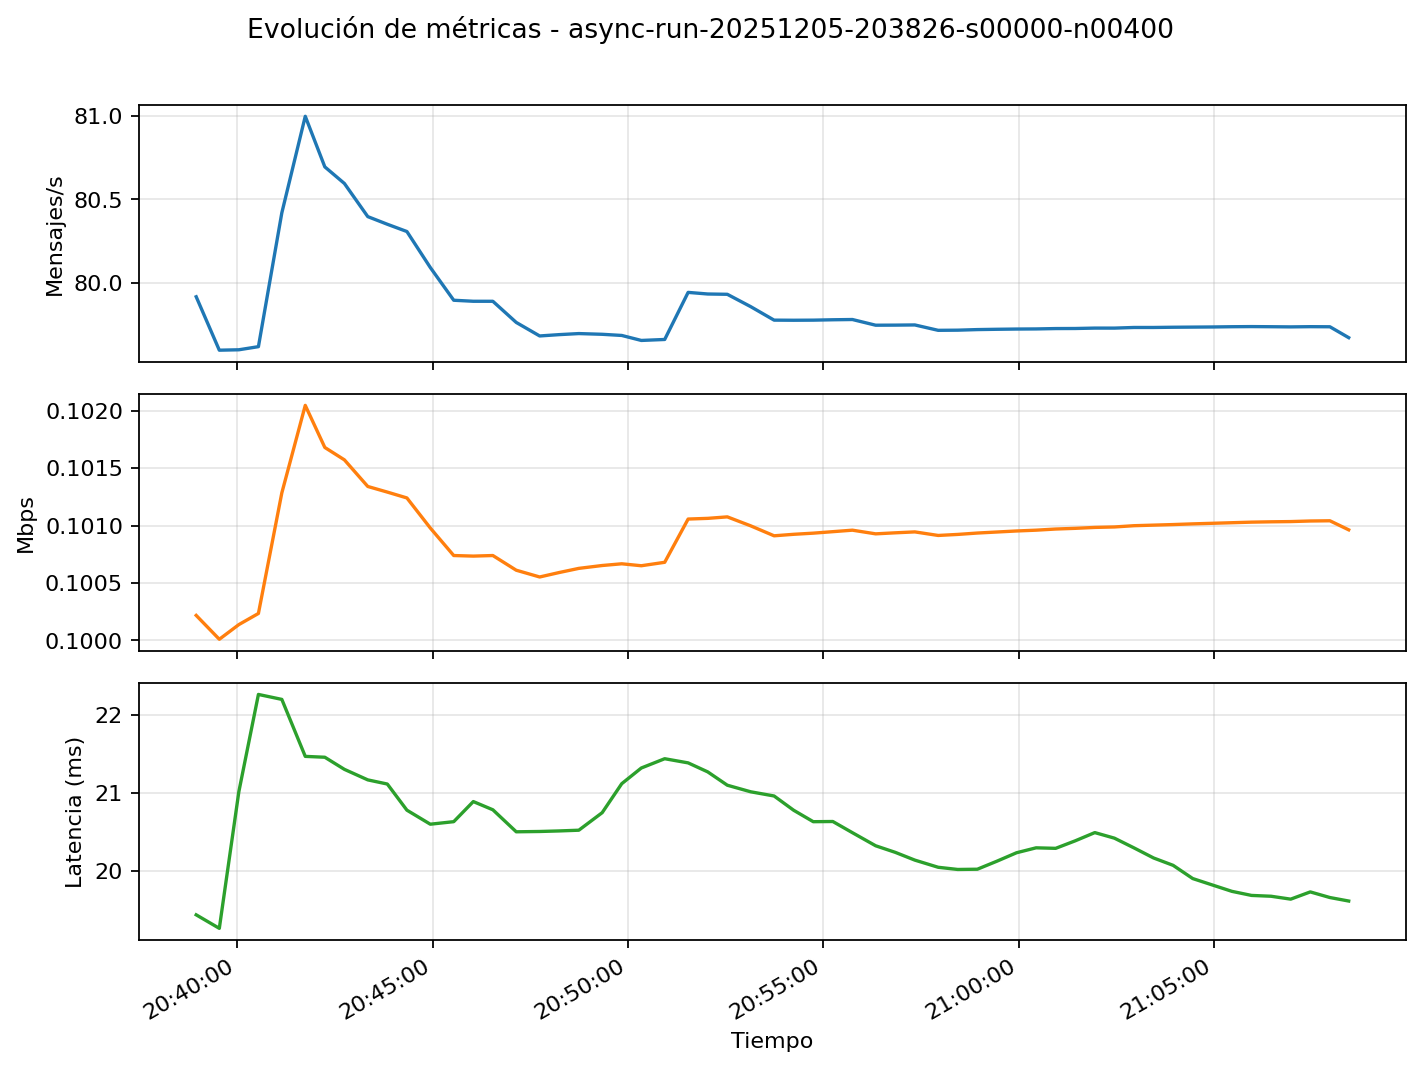
\includegraphics[width=\linewidth]{../data/metrics/reports/async-run-20251205-203826-s00000-n00400-overview.png}
  \caption{Evoluci\'on de m\'etricas del escenario async-run-20251205-203826-s00000-n00400.}
  \label{fig:esc-async-run-20251205-203826-s00000-n00400}
\end{figure}
\begin{table}[!t]
  \centering
  \caption{Resumen del escenario async-run-20251205-203826-s00000-n00400.}
  \label{tab:esc-async-run-20251205-203826-s00000-n00400}
  \begin{tabular}{@{}lrrrrr@{}}
    \toprule
    Sesi\'on & Nodos & Duraci\'on (s) & Mensajes & Lat. prom. (ms) & Throughput (msg/s)\\
    \midrule
    async-run-20251205-203826-s00000-n00400 & - & - & - & - & -\\
    \bottomrule
  \end{tabular}
\end{table}
\paragraph{Conclusiones autom\'aticas}
\begin{itemize}
  \item Datos insuficientes para generar m\'as conclusiones.
  \item Datos insuficientes para generar m\'as conclusiones.
  \item Datos insuficientes para generar m\'as conclusiones.
  \item Datos insuficientes para generar m\'as conclusiones.
\end{itemize}
\FloatBarrier
\subsubsection{Escenario async-run-20251205-203826-s00400-n00400 (400 dispositivos)}
\begin{table}[!t]
  \centering
  \caption{Resumen del escenario async-run-20251205-203826-s00400-n00400.}
  \label{tab:esc-async-run-20251205-203826-s00400-n00400}
  \begin{tabular}{@{}lrrrrr@{}}
    \toprule
    Sesi\'on & Nodos & Duraci\'on (s) & Mensajes & Lat. prom. (ms) & Throughput (msg/s)\\
    \midrule
    async-run-20251205-203826-s00400-n00400 & 400 & 1800 & 143455 & 20.285 & 79.844\\
    \bottomrule
  \end{tabular}
\end{table}
\paragraph{Conclusiones autom\'aticas}
\begin{itemize}
  \item Se ejercitaron aproximadamente 400 dispositivos.
  \item Entrega estable con p\'erdida <1\%.
  \item La latencia promedio se mantuvo baja para el escenario evaluado.
  \item El throughput medio fue de 79.84 msg/s.
\end{itemize}
\FloatBarrier
